
\cxset{style05/.style={
 chapter opening=any,
 chapter toc=true,
 name=Chapter,
 chapter color=black!90,
 numbering=arabic,
 number font-size=Large,
 number font-family=rmfamily,
 number font-weight=\normalfont\itshape,
 number color= black,
 number before=\kern0.5em,
 number dot=,
 number after=\hfill\hfill\par,
 number position= rightname,
 chapter shape=none,
 chapter display=block,
 chapter float=center,
 chapter font-family=rmfamily,
 chapter font-weight= itshape,
 chapter font-size=Large,
 chapter before=\hrule width \columnwidth \kern12.6pt \par\hfill,
 chapter after=,
 chapter color=black!90,
 chapter spaceout=none,
% handle margins and padding
 title margin top=10pt,
 title margin bottom=10pt,
 title before=,
 title after=\vskip12.6pt\hrule width \columnwidth,
 title font-family=rmfamily,
 title font-color=black!90,
 title font-weight=bfseries,
 title font-size=huge,
 chapter title align=centering,
 title font-shape = normal,
 header style= headings}}

\cxset{style05}
\chapter{Introduction to Style Five}\index{styles!style5}

\tcbset{width=\textwidth}
I think this style can be improved with a bit of color. You can experiment with it quite easily. The spacing on top of this style can also be adjusted to suit your typographical taste.
\medskip
\begin{figure}[ht]
\centering
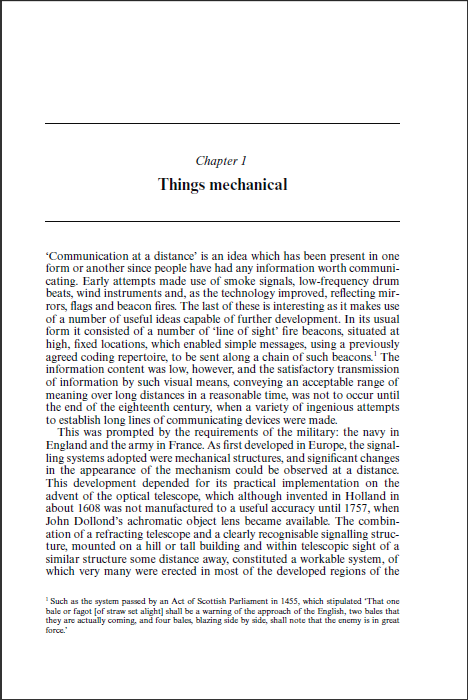
\includegraphics[width=0.6\textwidth]{./chapters/chapter05.png}
\end{figure}

%\section{General notes on rules}

LaTeX's default rules would normally give problems. Best is to use TeX's primitives to built them.

\index{rules!example color}

\begin{texexample}{}{}
\makeatletter
\hrule width 5cm \kern2.6\p@
AAAAAAAAAAAAAAAAAAAAA
\vskip2.6pt\hrule width 5cm
\medskip

Problem with LaTeX rules.

\rule{5cm}{0.4pt}\par
AAAAAAAAAAAAAAAAAAAAA\par%
\rule[6.5pt]{5cm}{0.4pt}

\def\rule{\@ifnextchar[\@rule{\@rule[\z@]}}
\def\@rule[#1]#2#3{%
 \leavevmode
 \hbox{%
 \setlength\@tempdima{#1}%
 \setlength\@tempdimb{#2}%
 \setlength\@tempdimc{#3}%
 \advance\@tempdimc\@tempdima%
 \vrule\@width\@tempdimb\@height\@tempdimc\@depth-\@tempdima}}

\def\thickrule{\leavevmode \leaders \hrule height 3pt \hfill \kern \z@}

{\color{teal}\hrule width 10.5cm height3pt \kern2.6\p@
    {{\color{black!80}\HUGE CHAPTER TITLE}}\vskip3pt
\hrule width 10.5cm height3pt}
\makeatother
\end{texexample}


\section{Images}

\begin{figure}[htbp]
\centering
\includegraphics[width=0.8\textwidth]{telegraphy}
\caption{Spread from the \textit{History of Telegraphy}, the caption is set left and the image is centered.}
\end{figure}
